\section{Het domeinmodel : klassendiagram en objectdiagram}

Zoals eerder al vermeld (hoofdstuk 1 - de objectgerichte visie) vormt het domeinmodel (synoniemen: business model, bedrijfsmodel) de ziel van de systeemontwikkeling. Hiervoor wordt typisch een klassendiagram opgesteld. Het is dan ook logisch diagram als eerste besproken wordt. Bovendien is het zo dat het klassendiagram de rode draad vormt in de systeemontwikkeling en in elke fase terug komt (deze terugkoppeling wordt bij de beschrijving van de andere modellen besproken).

Het \textbf{klassendiagram} is het meest uitgebreide diagram in UML en komt zoals eerder vermeld in de verschillende ontwikkelingsfasen terug. Daarin worden de klassen en de verschillende structurele, langdurige relaties die daartussen kunnen bestaan evenals de verschillende variaties die daarbij kunnen optreden, voorgesteld.

Een \textbf{klassendiagram} omvat het grootste deel van de statische structuur van het systeem. Met statisch wordt bedoeld dat een klassendiagram op elk punt in de levenscyclus betekenisvol is en dus niet verandert naargelang het moment tijdens de systeem- levenscydus dat ze bekeken wordt.

Een \textbf{klassendiagram} toont de statische structuur van de klassen. Een klasse stelt iets (object) voor dat betekenis heeft in de werkelijkheid. In het klassendiagram worden ook de structurele verbanden tussen deze objecten voorgesteld.

Een \textbf{objectdiagram} is een variant op het klassendiagram en maakt gebruik van bijna identieke symbolen. Net zoals een object een instantiatie is van een klasse, is het objectdiagram een instantiatie van het klassendiagram.
Het grote verschil tussen beide is dat het klassendiagram geldig is doorheen de ganse systeemontwikkeling en -levenscyclus, terwijl het objectdiagram een momentopname weergeeft van de uitvoering van het systeem.

Zoals eerder vermeld worden hiervoor bijna identieke symbolen gebruikt als bij het klassendiagram met uitzondering van het volgende: de objectnamen worden vooraf gegaan door de naam van de klassen waaruit ze geïnstantieerd zijn. De klassennamen worden onderstreept en alle instanties van een associatie worden weergegeven. Bij de uitwerking van de verschillende concepten van het klassendiagram zullen de overeenkomsten en verschillen met het objectdiagram vermeld worden.

Aangezien het klassendiagram de representatie is van de dingen waarvan de systeem- ontwikkelaar vertrekt, zal een klassendiagram steeds opgesteld worden, het objectdiagram daarentegen wordt enkel uitgewerkt als men een situatie wil illustreren/ verduidelijken met een concreet voorbeeld.
Het klassendiagram vormt de rode draad doorheen de softwareontwikkeling: telkens als bepaalde diagrammen verder uitgewerkt worden, wordt teruggekoppeld naar het klassendiagram. Natuurlijk zijn het ook de klassen van het laatste versie klassendiagram waarvoor uiteindelijk de klassendefinities geschreven zullen worden.
\newpage
\subsection{Klassendiagram / objectdiagram: onderdelen}

Een klassendiagram bestaat in eerste instantie uit klassen: een klasse beschrijft een verzameling objecten in een systeem die een gelijkwaardige rol of rollen hebben, of m.a.w. een klasse is een sjabloon voor het maken van objecten.

Hierbij onderscheidt men een aantal "soorten" klassen (deze klassen overlappen elkaar):

\begin{itemize}
    \item tastbare dingen uit de wereld, bv. een klant, een boek, een cursus...
    \item rollen : een lid van de bibliotheek, een student... 
    \item gebeurtenissen : aankomst, vertrek,...
    \item interacties : samenkomst, kruising,...
\end{itemize}

Een object daarentegen is een concreet voorkomen van een klasse, een element uit de verzameling die aangeduid wordt door de klasse, bv. deze cursustekst

Klassen en objecten hebben eigenschappen, deze eigenschappen noemt men de attributen. Zo heeft een cursustekst bv. de attributen: aantalBladzijden, moeilijkheidsgraad, enz.

Een speciaal attribuut is het afgeleid attribuut. Dergelijk attribuut kan je afleiden uit andere attributen. Men geeft aan dat het handelt over een afgeleid attribuut door een slash (" / ") te plaatsen voor het attribuut in kwestie.

Bijvoorbeeld, het attribuut leeftijd kan men afleiden indien men de geboortedatum van een persoon heeft opgenomen.

Verder hebben klassen en objecten operaties, met name hun gedragskenmerken. Deze bepalen het gedrag dat objecten van die klasse kunnen vertonen.

Een klasse wordt voorgesteld door een rechthoek met daarin 3 compartimenten.

\begin{itemize}
    \item De naam van de klasse vind je in het eerste compartiment en wordt centraal genoteerd met een hoofdletter. Indien de naam van de klasse uit twee of meer woorden bestaat, schrijf je die woorden aan elkaar waarbij het volgende woord opnieuw met een hoofdletter geschreven wordt.
    \item In het tweede compartiment noteert men de attributen van de klasse. Een klasse kan 0, 1 of meerdere attributen hebben. Elk attribuut wordt geschreven in kleine letters. Indien de naam van het attribuut uit meerdere woorden bestaat, dan schrijft men die woorden aan elkaar waarbij elk volgend woord met een hoofd letter begint.
    \item Bijkomend kan men voor elk attribuut aangeven van welk type dit attribuut is.
    \item Tenslotte worden de operaties genoteerd. Hierbij gelden dezelfde afspraken als bij een attribuut: de naam van een operatie wordt in kleine letters genoteerd. Indien de operatienaam uit meerdere woorden bestaat, schrijf je die woorden aan elkaar en elk volgend woord begint met een hoofdletter. Achter de operatienaam kan men tussen haakjes extra informatie opnemen: men kan er de parameters plaatsen waarop de operatie werkt, plus het parametertype. Indien het handelt over een functie geef je aan welke waarde door de functie teruggeven wordt en welk type deze waarde heeft.
\end{itemize}

%afbeelding nog plaatsen

\begin{center}
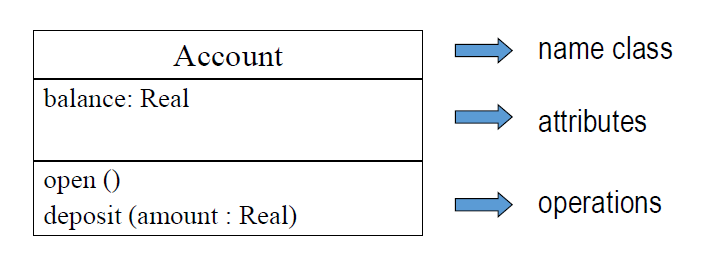
\includegraphics[width=4in]{img/klas1}%
\end{center}

De conventies die gelden voor een object zijn analoog aan deze van de klasse : ook het object wordt in een rechthoek getekend.

%afbeelding nog plaatsen

\begin{center}
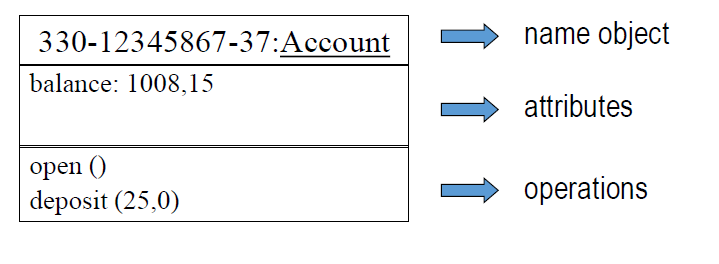
\includegraphics[width=4in]{img/klas2}%
\end{center}

De naam van het object verschijnt bovenaan maar men geeft bijkomend aan van welke klasse dit een object is. De objectnaam wordt in kleine letters genoteerd (ook de eerste letter) en na het dubbele punt verschijnt de klassennaam die onderlijnd is.
Aangezien het object een concreet voorkomen is van de klasse, geeft men voor elk attribuut de concrete waarde.
\newpage
\subsection{klassendiagram en objectdiagram: concepten}

De volgende concepten zijn van belang bij het opmaken van klasse- en objectdiagrammen:

\subsubsection{associatie}

Een associatie geeft de onderlinge relatie aan tussen twee klassen, bv. de klasse "Persoon" die door de associatie "werktBij" verbonden is met de klasse "Bedrijf". Een associatie wordt genoteerd als een lijn tussen de twee klassen die verbonden worden door de associatie, waarbij de naam van de associatie bij de associatie geplaatst wordt.

%afbeelding nog plaatsen

\begin{center}
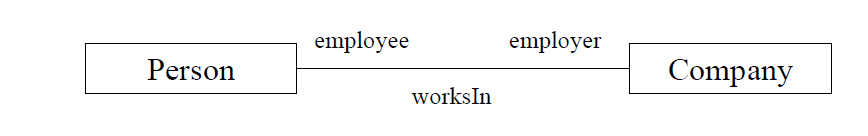
\includegraphics[width=4in]{img/ass1}%
\end{center}

Een klasse A is geassocieerd met een klasse B indien :

\begin{itemize}
    \item Een object van klasse A een bericht naar een object van klasse B stuurt
    \item Een object van klasse A een object van klasse B creëert
    \item Een object van klasse A een attribuut heeft waarvan de waarden objecten van klasse B zijn of verzamelingen objecten van klasse B
    \item Een object van klasse A een bericht ontvangt met een object van klasse B als argument.
\end{itemize}

Of met andere woorden : een klasse A moet geassocieerd zijn met een klasse B indien een object van klasse A bekend moet zijn met een object van klasse B.

\subsubsection{link}

Zoals een object een instantie (concreet voorkomen) is van een klasse, zo heeft een associatie ook instanties.

%afbeelding nog plaatsen

\begin{center}
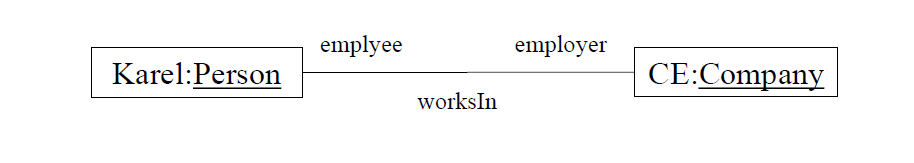
\includegraphics[width=4in]{img/link1}%
\end{center}

Als een bepaald persoon, bv. Karei werkt in een bepaald bedrijf, bv. CE en we stellen deze relatie voor, dan spreekt men van een link. Een link wordt dus eveneens voorgesteld door een lijn, maar een link verbindt twee objecten in een objectdiagram.
Naar analogie met de objectnaam wordt ook de naam van de link onderlijnd.
\newpage
\subsubsection{rol}

Als een klasse met een andere klasse geassocieerd wordt, speelt elk van die klassen meestal een rol in die associatie (afhankelijk van de context). Je kan deze rollen in het diagram opnemen door de naam van de rol bij de lijn te schrijven naast de klasse die de betreffende rol speelt.

%afbeelding nog plaatsen

\begin{center}
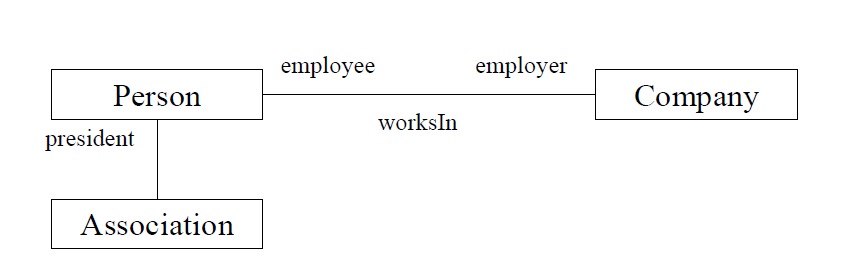
\includegraphics[width=4in]{img/rol1}%
\end{center}

Klassen kunnen via meerdere associaties met elkaar verbonden worden en op die manier ook verschillende rollen spelen.

Voorbeeld. Persoon is werknemer bij een bepaald bedrijf, maar kan ook voorzitter zijn van een bepaalde club. Dan speelt die persoon meerdere rollen.

\subsubsection{associatieklasse}

Indien een associatie attributen en/of operaties heeft, spreekt men van een associatieklasse. Een associatieklasse noteren, gebeurt op dezelfde manier als een gewone klasse, maar een stippellijn verbindt de associatieklasse met de associatielijn. Op het moment dat een link gelegd wordt tussen objecten van beide klassen, wordt automatisch ook een object van de associatieklasse aangemaakt.
Een associatieklasse kan op zich associaties hebben naar andere klassen.

%afbeelding nog plaatsen

\begin{center}
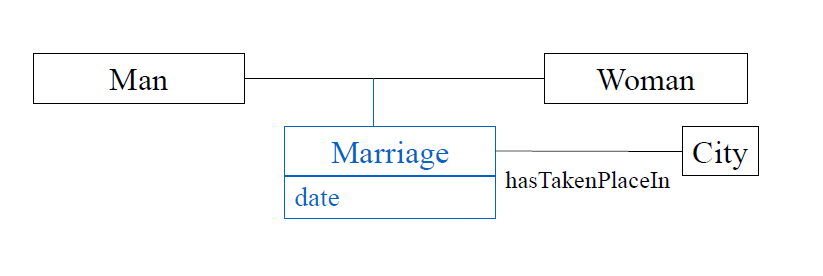
\includegraphics[width=4in]{img/asscl1}%
\end{center}
\newpage
\subsubsection{multipliciteit}

De multipliciteit van de associatie geeft aan met hoeveel instanties van de geassocieerde klasse een instantie van een klasse geassocieerd kan zijn. Deze multipliciteit geldt gedurende de ganse levenscyclus van het systeem.

%afbeelding nog plaatsen

\begin{center}
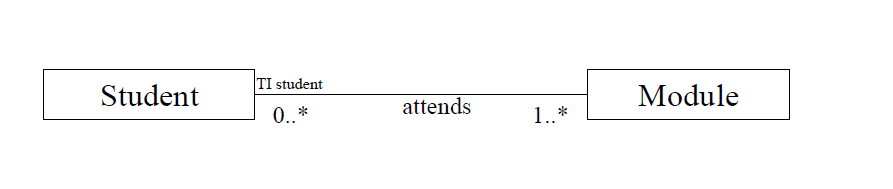
\includegraphics[width=4in]{img/mul1}%
\end{center}

Om een multipliciteit op te geven kan men gebruik maken van een exact getal (bv. 5), een getallenbereik (tussen 0 en 5) of een willekeurig, ongespecificeerd getal, dat aangeduid wordt door een *

Er zijn veel verschillende multipliciteiten mogelijk :

\begin{itemize}
    \item één-op-één (1 op 1)
bv. 1 echtgenoot is gehuwd met 1 echtgenote
    \item één-op-veel (1 op *)
bv. 1 leraar geeft les aan veel leerlingen
    \item één-op-één of meer (1 op 1..*)
bv. 1 bankbediende bedient 1 tot meer klanten
    \item één-op-nul of één (1 op 0..1)
bv. 1 huis heeft 0 of 1 schoorsteen
\item één-op-bepaald aantal (1 op 3) bv. 1 driewieler heeft 3 wielen
    \item één-op-een bepaald interval (1 op 5.. 10) bv. 1 reeks bevat 20 tot 32 studenten
    \item ...
\end{itemize}

\subsubsection{afgeleide associatie}

Indien een klasse A geassocieerd is met een klasse B en klasse B heeft op zijn beurt een associatie naar klasse C, dan kan men een afgeleide associatie tussen klasse A en klasse C opnemen. Deze associatie kan dus afgeleid worden uit andere associaties.

%afbeelding nog plaatsen

\begin{center}
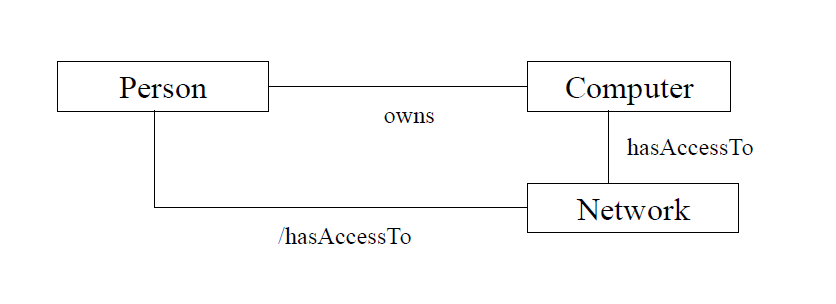
\includegraphics[width=4in]{img/dera1}%
\end{center}

Dergelijke afgeleide associatie wordt genoteerd conform de afspraken m.b.t. de associaties maar men iaat de naam voorafgaan door een slash ("/")

Opmerking. Zelfde notatie als afgeleid attribuut.

\subsubsection{gekwalificeerde associatie}

Als de multipliciteit van een associatie één-op-veel is, rijst vaak de vraag hoe je dingen kan opzoeken. Als een object van de ene klasse een bepaald object van een andere klasse moet kiezen, moet de eerste klasse op een specifiek attribuut vertrouwen om het juiste object te vinden. Dit attribuut is een identificatie.
In UML noemt men deze identificator de kwalificator. Deze kwalificator wordt voorgesteld door een kleine rechthoek die vastzit aan de klasse die het opzoekwerk verricht.

%afbeelding nog plaatsen

\begin{center}
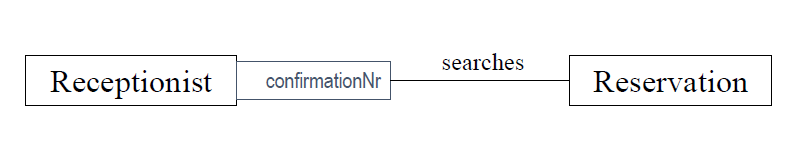
\includegraphics[width=4in]{img/qa1}%
\end{center}

\subsubsection{reflexieve associatie}

Soms is een klasse met zichzelf geassocieerd. Dit gebeurt indien een klasse objecten heeft die allerlei rollen kunnen spelen. Zo zal bv. een Persoon een associatie "is gehuwd met" hebben met een Persoon, deze klasse kan immers de rol Echtgenoot en de rol Echtgenote hebben.

%afbeelding nog plaatsen

\begin{center}
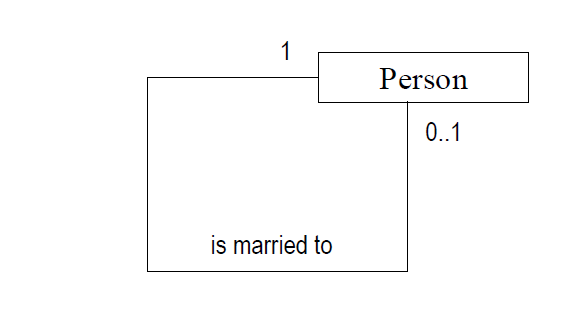
\includegraphics[width=4in]{img/ra1}%
\end{center}

Een reflexieve associatie wordt volledig analoog met andere associaties getekend, nl. een lijn tussen de twee klassen, in dit geval dus een lijn die vertrekt en toekomt in dezelfde klasse. Ook hier kan men de rollen aanduiden die de klasse heeft in de associatie.

\subsubsection{toegankelijkheid}

De toegankelijkheid is van toepassing op attributen en operaties en geeft aan in welke mate andere klassen attributen en operaties van een bepaalde klasse kunnen gebruiken.

Er zijn drie niveaus van toegankelijkheid mogelijk :

\begin{itemize}
    \item public (publiek) :
de bruikbaarheid strekt zich uit tot de andere klassen.
Een publiek attribuut of operatie wordt voorgesteld door "+"
    \item private (privaat) :
alleen de oorspronkelijke klasse kan het attribuut of de operatie gebruiken.
Een privaat attribuut of operatie wordt voorgesteld door " - "
    \item protected (beschermd) :
de bruikbaarheid is beperkt tot klassen die erven van de oorspronkelijke klasse (voor overerving cf. infra)
Een beschermd attribuut of operatie wordt voorgesteld door "\#"
\end{itemize}

Let op. De toegankelijkheid is niet hetzelfde als de zichtbaarheid!
De beslissing om een attribuut of een operatie public, private of protected te maken, stel je best zo lang mogelijk uit.

\subsubsection{Generalisatie}

Met generalisatie wordt bedoeld dat er een hiërarchie bestaat tussen een aantal klassen, waarbij het zo is dat één klasse de ouderklasse is, waarvan andere klassen overerven. Dit betekent dat de kind-klassen de attributen en operaties van de ouderklasse, die algemener is, overnemen en hierbij nog eventueel extra attributen of operaties toevoegen. Denk aan het principe van de typering (zie eerder)! De ouderklasse noemt men de superklasse, de kind-klassen zijn de subklassen.

%afbeelding nog plaatsen

\begin{center}
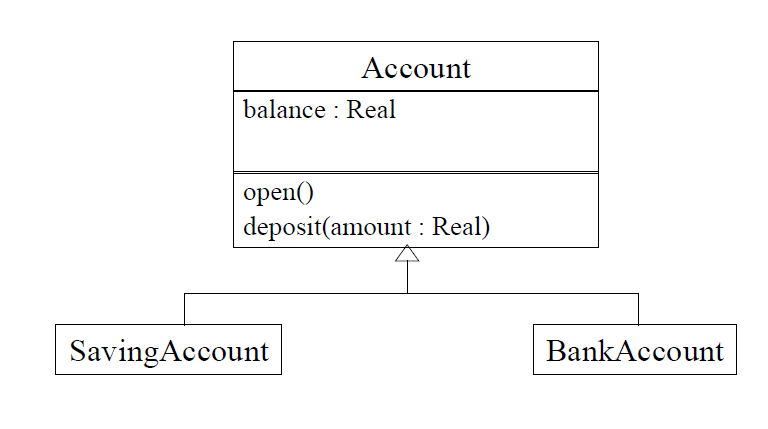
\includegraphics[width=4in]{img/con1}%
\end{center}

Voorbeeld. Nemen we de klasse Rekening, deze heeft een saldo, men kan de Rekening openen en men kan een bedrag terugtrekken. Deze algemene kenmerken en operaties komen eveneens voor in de subklassen Bankrekening en Spaarrekening, maar een bankrekening kan bv. een negatief saldo hebben, dit is bij een spaarrekening onmogelijk. Op een bankrekening moet men debet intresten betalen, op een Spaarrekening niet.

In object-oriëntatie spreekt men van overerving, UML gebruikt de term "generalisatie".

De generalisatie wordt getoond door een lijn die de ouderklasse met de kind- klasse verbindt, op het deel van de lijn dat met de ouderklasse verbonden is, moet een open driehoekje getekend worden dat verwijst naar de ouderklasse.

Voorbeeld, een superklasse "Rekening" die gespecialiseerd wordt in twee subklassen "Spaarrekening" en "Bankrekening"..

De attributen en operaties die door de subklassen geërfd worden moeten in de subklassen niet meer vermeld worden aangezien deze al verschijnen in de superklasse. De extra attributen en/of operaties van de subklassen worden natuurlijk wel nog vermeld in de subklassen.

Let op voor het principe van typering: eens een object gecreëerd is, kan het niet meer van type veranderen. Denk hierbij aan het eerder aangehaalde voorbeeld van de verschillende ruimtes in een hotel: een kamer kan op een ander moment ook gebruikt worden als vergaderruimte, enz.
\newpage
\subsubsection{meervoudige overerving}

Indien een klasse meer dan één ouder heeft, spreekt men over een meervoudige overerving. In het geval een klasse slechts één ouder heeft, handelt het over een enkelvoudige overerving.

Voorbeeld, een telefax kan gezien worden als subklasse van zowel een Fax als van een Telefoon.

Let op. Een opmerkingen die regelmatig ter sprake komt bij meervoudige overerving is dat als bepaalde methodes bij beide supertypes gedefinieerd zijn op een andere manier, de vraag rijst welke methode overgeërfd moet worden. Het antwoord hierop is vrij eenvoudig: in het subtype moet deze methode geherdefinieerd worden.

\subsubsection{herhaalde overerving}
Men spreekt over herhaalde overerving indien meerdere superklassen van één subklasse op zich samen weer één superklasse hebben.

Voorbeeld, in bovenstaande meervoudige overerving kan men de superklassen Fax en Telefoon zien als subklassen van de superklasse TelecommunicatieApparaat.

%afbeelding nog plaatsen

\begin{center}
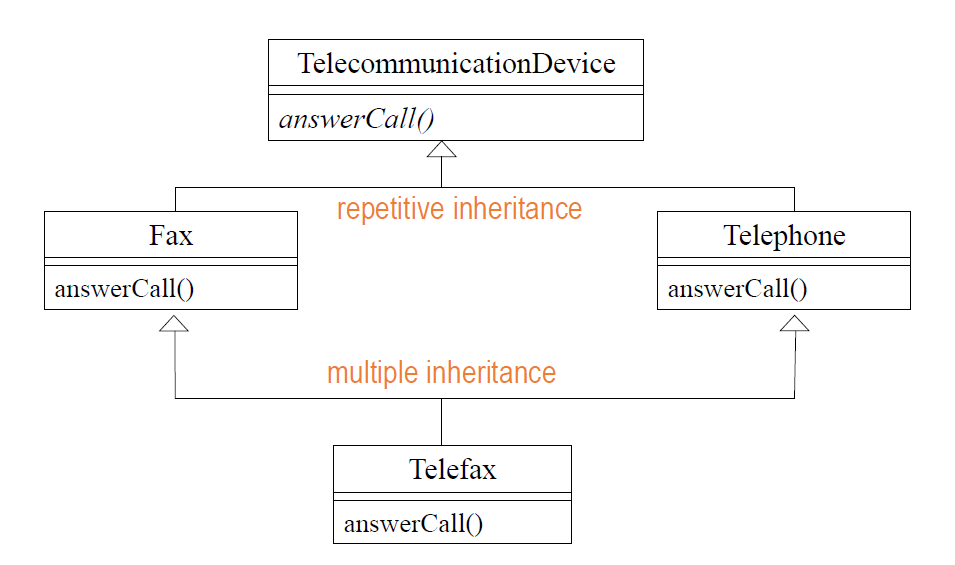
\includegraphics[width=4in]{img/con2}%
\end{center}
\newpage
\subsubsection{abstracte klasse}

Een klasse waarin bepaalde onderdelen nog niet gedefinieerd zijn, wordt een abstracte klasse genoemd. Uit een abstracte klasse kunnen dus nooit objecten geïnstantieerd worden!
Een abstracte klasse is altijd een superklasse in een generalisatie, aangezien dergelijke klasse nooit geïnstantieerd zal worden. In de subklassen worden dan de niet gedefinieerde elementen gedefinieerd en dan kunnen wel objecten geïnstantieerd worden.

Zo ook is een abstracte operatie een operatie die niet geïnstantieerd wordt, die m.a.w. geen methodedefinitie heeft.

%afbeelding nog plaatsen

\begin{center}
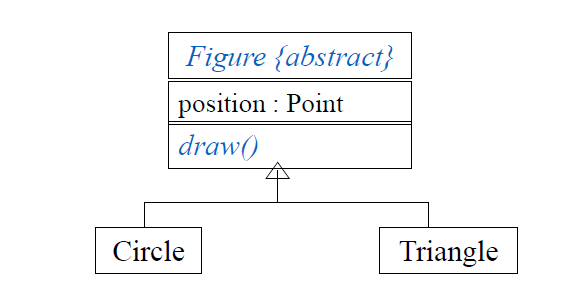
\includegraphics[width=4in]{img/abs1}%
\end{center}

Om een abstracte klasse aan te duiden, gebruikt men het pictogram van een klasse maar de naam van de klasse wordt in cursief gezet. Ook een abstracte operatie wordt analoog, in cursief dus, aangeduid.

\subsubsection{interface}

Indien je een aantal operaties voor een klasse ontwikkelt die je wil hergebruiken in andere klassen, kan je gebruik maken van een interface. Via deze interface kan beschreven worden hoe instanties van een klasse benaderd kunnen worden door andere objecten.

Een interface is nl. een verzameling operaties die één of ander aspect van het gedrag van een klasse specificeert waarbij deze verzameling operaties aan andere klassen gepresenteerd worden.
Of m.a.w. een interface is een verzameling operaties die door een klasse worden uitgevoerd.

%afbeelding nog plaatsen

\begin{center}
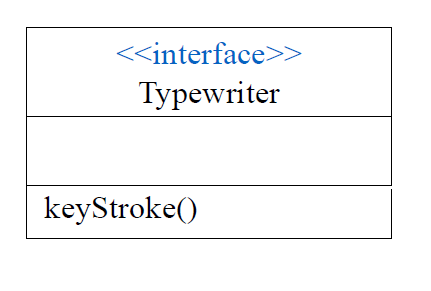
\includegraphics[width=4in]{img/int1}%
\end{center}

Een interface wordt op dezelfde manier genoteerd als een klasse, nl. door een rechthoek. Aangezien een interface echter geen attributen heeft, zullen deze niet verschijnen in een interface.
Bijkomend wil men natuurlijk wel het verschil maken tussen een klasse en een interface, dit gebeurt door in de interfacenaam het stereotype

\begin{center}
«interface»
\end{center}

toe te voegen. Soms wordt een interface ook voorgesteld door een bolletje.

Een klasse is gerelateerd aan een interface via realisatie, om dit aan te duiden wordt een stippellijn getekend met een pijl die naar de interface wijst.

%afbeelding nog plaatsen

\begin{center}
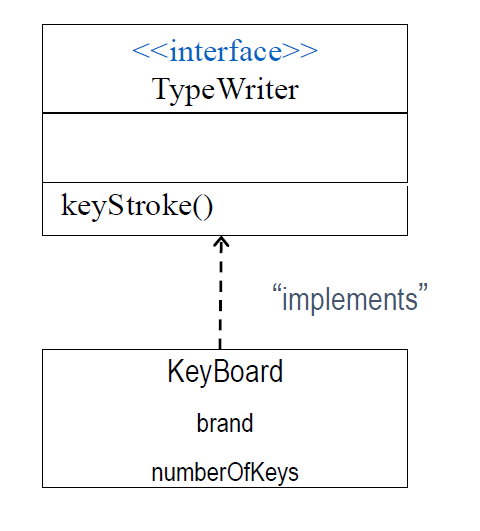
\includegraphics[width=4in]{img/int2}%
\end{center}

\newpage
\subsubsection{aggregatie en compositie : (mogelijke examenvraag)}

Aggregatie en compositie zijn soorten associaties, maar in plaats van enkel te tonen dat twee klassen geassocieerd zijn, wordt door een aggregatie en door een compositie aangegeven dat het handelt over een speciaal soort associatie, nl. de associatie "is onderdeel van".

De aggregatie en de compositie geven beide aan dat een object van klasse A een onderdeel is van een object van klasse B, bijvoorbeeld een fiets bestaat uit een wiel, een frame, ...

De associatie moet geen naam krijgen, aangezien die gekend is door het type associatie dat men voorstelt.

Het \textbf{verschil} tussen een aggregatie en een compositie bestaat in de mate waarin de onderdelen vast zitten in het geheel: bij een \textbf{compositie} is het geheel nadrukkelijk eigenaar van de delen, als het geheel wordt verwijderd, dan vallen ook de delen weg. Dit is het gevolg van het feit dat de componenten in een compositie bij precies één geheel horen.

In een aggregatie daarentegen is het verband tussen het onderdeel en het
geheel veel losser : het onderdeel hoort wel tot het geheel maar dit kan veranderd worden waardoor het onderdeel tot een ander geheel zal horen.

%afbeelding nog plaatsen

\begin{center}
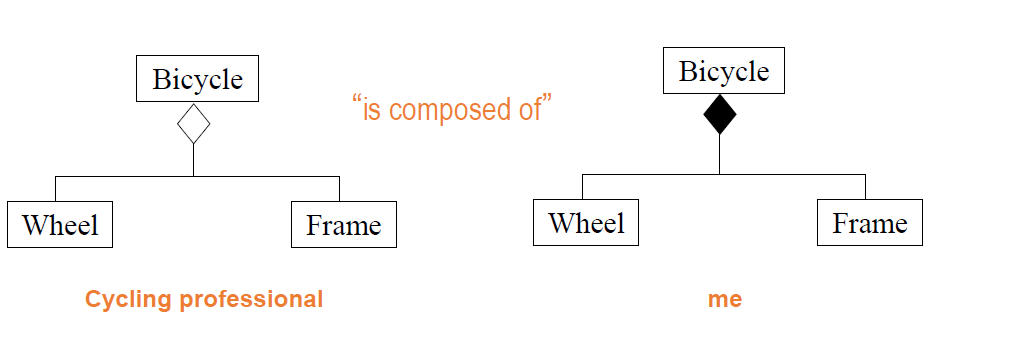
\includegraphics[width=4in]{img/aggcom}%
\end{center}

Neem bvb. de compositie die bestaat tussen een fiets en zijn onderdelen "wiel" en "frame". Dit zijn delen van de fiets, indien het wiel stuk is, kan je niet meer rijden en is het geheel dus verdwenen.
Dergelijk verband bestaat er niet voor wielertoeristen die voor een fietstochtje een frame, enkele wielen, ... meenemen. Naargelang de weersomstandigheden wordt één bepaald type wiel genomen en op een ander moment zal de fiets samengesteld worden uit andere wielen. In dit geval kan men spreken over een aggregatie tussen de fiets en zijn onderdelen.
Een aggregatie wordt voorgesteld door een open ruit aan het geheel, de compositie door een gevulde ruit.

\subsubsection{constraints}

In een klassenpictogram kan men heel wat informatie over de klassen specificeren, soms is het echter nodig om een extra beperking op te nemen, nl. een regel die voor de klasse geldt. Deze regels worden contraints (beperkingen) genoemd.

%afbeelding nog plaatsen

\begin{center}
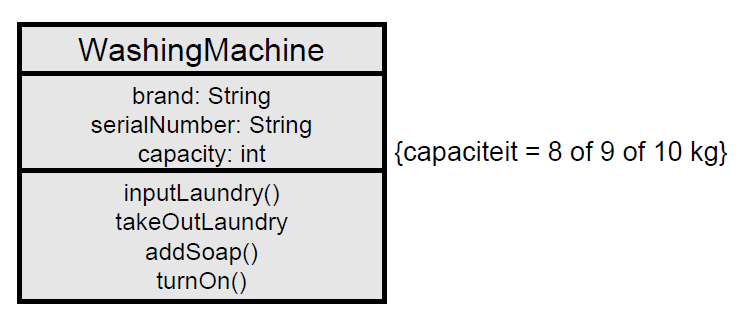
\includegraphics[width=4in]{img/const1}%
\end{center}

Men noteert een constraint door de tekst die de beperking aangeeft, op te nemen tussen accolades of door deze toe te voegen in een notebox (notitie). UML kent een andere, veel formelere, manier om beperkingen toe te voegen die de definities explicieter maken, nl. OCL, de Object Constraint Language.

\subsection{klassendiagram en objectdiagram: werkwijze}

Het klassendiagram wordt als volgt opgesteld (volgens de regels van OMT):

\begin{itemize}
    \item Identificeer alle mogelijke kandidaat klassen
    
    Uit de probleemomschrijving selecteert men alle zelfstandige naamwoorden, aangevuld met de informatie die men distilleert uit brainstormsessies met alle betrokkenen.
    \item Selecteer de klassen uit de opgestelde lijst
    
    Uit de bekomen lijst worden de relevante klassen weerhouden (geen redundante, vage niet-kwantificeerbare klassen, geen klassen die eigenlijk attributen zijn, enz.)
    \item Maak een model dictionary
    
    Vervolgens stel je een model dictionary op met alle klassen, attributen en operaties die tot nog toe duidelijk zijn
    \item Identificeer associaties
    
    De paren van klassen die geassocieerd moeten worden, worden geïdentificeerd en je voegt de multipliciteiten en eventueel de rollen toe.
    \item Identificeer attributen
    
    Vooralle klassen worden alle attributen genoteerd die noodzakelijk zijn voor het te ontwikkelen systeem.
    \item Identificeer operaties
    
    Vervolgens ga je voor alle klassen na welke operaties toegevoegd moeten worden.
    \item Generaliseer met behulp van overerving
    
    Op dit moment ga je op zoek naar overeenkomsten tussen de verschillende klassen om eventuele superklassen en subklassen te identificeren.
    
    De gemeenschappelijke attributen en operaties worden in de superklasse genoteerd, de specifieke blijven in de subklassen.

\item Maak OCL-constraints

Eventuele bedrijfsregels en beperkingen worden toegevoegd.

\item Groepeer klassen eventueel in packages

Indien je werkt aan een groot, complex systeem, ga je op dit moment de klassen onderverdelen in packages, zodanig dat je overzichtelijke delen bekomt.
\item Itereer over de gedane stappen

Op basis van de onvolledigheden in de uitgewerkte oplossing worden aanpassingen aangebracht in het systeem door de hierboven opgesomde stappen opnieuw uit te voeren.
\end{itemize}

